\documentclass[a4paper, 12pt]{article}		% general format

%%%% Charset
\usepackage{cmap}							% make PDF files searchable and copyable
\usepackage[utf8x]{inputenc}				% accept different input encodings
\usepackage[T2A]{fontenc}					% russian font
\usepackage[russian]{babel}					% multilingual support (T2A)

%%%% Graphics
\usepackage[dvipsnames]{xcolor}			% driver-independent color extensions
\usepackage{graphicx}						% enhanced support for graphics
\usepackage{wrapfig}						% produces figures which text can flow around

%%%% Math
\usepackage{amsmath}						% American Mathematical Society (AMS) math facilities
\usepackage{amsfonts}						% fonts from the AMS
\usepackage{amssymb}						% additional math symbols

%%%% Typograpy (don't forget about cm-super)
\usepackage{microtype}						% subliminal refinements towards typographical perfection
\linespread{1.3}							% line spacing
\usepackage[left=2.5cm, right=1.5cm, top=2.5cm, bottom=2.5cm]{geometry}
\setlength{\parindent}{0pt}					% we don't want any paragraph indentation
\usepackage{parskip}						% some distance between paragraphs

%%%% Tables
\usepackage{tabularx}						% tables with variable width columns
\usepackage{multirow}						% for tabularx
\usepackage{hhline}							% for tabularx

%%%% Graph
\usepackage{tikz}							% package for creating graphics programmatically
\usetikzlibrary{arrows}						% edges for tikz

%%%% Other
\usepackage{url}							% verbatim with URL-sensitive line breaks
\usepackage{fancyvrb}						% sophisticated verbatim text (with box)
%------------------------------------------------------------------------------

\begin{document}

%------------------------------------------------
\begin{titlepage}
\thispagestyle{empty}

\begin{center}
Санкт-Петербургский политехнический университет Петра Великого\\
Институт Информационных Технологий и Управления \\*
Кафедра компьютерных систем и программных технологий \\*
\hrulefill
\end{center}

\vspace{15em}

\begin{center}
\Large Отчёт по лабораторной работе №1\\по предмету «Администрирование компьютерных сетей» \\
\end{center}

\vspace{1em}

% \linebreak
\begin{center}
\textsc{\textbf{Виртуальное макетирование компьютерных сетей}}
\end{center}

\vspace{20em}

\begin{flushleft}
Работу выполнил студент гр. 53501/3 \hrulefill Мартынов С. А. \\
\vspace{1.5em}
Работу принял преподаватель \hrulefill Малышев И. А. \\
\end{flushleft}

\vspace{\fill}

\begin{center}
Санкт-Петербург \\
2015
\end{center}

\end{titlepage}
%------------------------------------------------
\setcounter{page}{2}
\tableofcontents

%------------------------------------------------------------------------------
\newpage
\section*{Введение}
\addcontentsline{toc}{section}{Введение}

Настоящая лабораторная работа расчитана на индивидуальное выполнение, с целью развития базовых навыков планирования и запуска сетей на основе TCP/IP протокола. Субьектом исследования будет являться полунатуральный эмулятор корпоративной компьютерной сети (ККС), который будет построен в виртуальном окружении.

Инструментальной платформой полунатурного эмулятора ККС служит программный продукт Oracle VM VirtualBox, разработанный компанией Oracle (ранее Sun Microsystems и Innotek). На момент написания отчёта (апрель 2015 года) актуальной являлась версия VirtualBox 4.3.26.

Ключевыми особенностями программы является:
\begin{itemize}
\item Кроссплатформенность;
\item Модульность;
\item Поддержка USB 2.0;
\item Поддержка 64-битных гостевых систем;
\item Поддержка SMP на стороне гостевой системы;
\item Встроенный RDP-сервер;
\item Поддержка аппаратного 3D-ускорения (OpenGL, DirectX);
\item Поддержка образов жёстких дисков VMDK, VHD и прочее;
\item Поддержка цепочки сохраненных состояний виртуальной машины (snapshots);
\item Поддержка iSCSI;
\item Поддержка виртуализации аудиоустройств;
\item Поддержка Shared Folders для простого обмена файлами между хостовой и гостевой системами;
\item Поддержка интеграции рабочих столов (seamless mode);
\item Мультиязычный интерфейс.
\end{itemize}

Отдельно стоит указать про сетевые возможности. VirtualBox обеспечивает следующие типы подключения:
\begin{itemize}
{\item Not attached (Сеть не подключена)

Режим в котором VirtualBox «сообщает» виртуальной машине, что сетевой интерфейс установлен, но кабель не подключен и сеть не доступна. Рекомендуется для отладки сетевых приложений.}

{\item Network Address Translation (NAT)

Наиболее простой способ получить доступ к внешней сети из виртуальной машины. Обычно не требует настроек, данный режим устанавливается для виртуальных сетевых интерфейсов по умолчанию. Виртуальная машина подключается к интернету, как реальная в локальной сети через маршрутизатор (шлюз, которым является для нее VirtualBox), но в данном режиме гостевая ОС не доступна для внешней сети.

Виртуальная машина получает IP адрес и настройки локальной сети через DHCP встроенный в VirtualBox. IP адрес хоста и гостя обычно находятся в разных подсетях. Первый сетевой интерфейс входит в сеть 10.0.2.0, второй в 10.0.3.0 и так далее. 

В данном режиме хосту не доступна внутренняя сеть и сетевые сервисы в виртуальной машине. Однако возможно используя перенаправление портов (port forwarding) сделать доступными сервисы виртуальной машины для хоста и других систем внешней сети - VirtualBox "слушает" порты на хосте и пересылает пакеты на виртуальный интерфейс. Для этого нужно учесть и распределить номера портов которые должен обрабатывать хост, а какие виртуальная машина (не всегда возможно использовать зарезервированные номера портов для нужного сервиса).


NAT имеет четыре существенных ограничения о которых нужно знать:
	\begin{itemize}
	\item Слабая поддержка ICMP, которая требуется многим программам мониторинга и отладки (например ping 	или tracerouting);
	\item Госевые ОС не прослушивают постоянно широковещательные рассылки, это сделано для улучшения производительности (как следствие, протокол NetBios не всегда корректно работает);
	\item Не поддерживаются некоторые протоколы, такие как GRE (это означает, что VPN (PPTP от Microsoft) не может использоваться);
	\item На Unix-based хостах (Linux, Solaris, MacOS X и т.п.) невозможно настроить порты ниже 1024 из приложений которые не запущены с правами суперпользователя (root). 
	\end{itemize}
}

{\item Bridged networking (Сетевой мост)

В этом режиме VirtualBox использует драйвер сетевого устройства в системе хоста для обработки пакетов с реального сетевого интерфейса. Этот драйвер называют «net filter» (сетевой фильтр). Он позволяет перехватывать пакеты из физической сети и создавать новые «программные» сетевые интерфейсы. При использовании виртуальной машиной такого программного интерфейса, возможна работа этого виртуального интерфейса через сетевой интерфейс хоста. Хост может принимать и посылать данные гостевой ОС, что означает что ВМ может взаимодействовать с другими устройствами физической сети.
}

{\item Internal networking (Внутренняя сеть)


Внутренняя сеть подобна обычной физической сети , в которой виртуальная машина может непосредственно общаться с внешним миром. Однако, "внешний мир" ограничен другими виртуальными машинами, которые соединяются к той же самой внутренней сети. Есть несколько оснований использовать данное решение:
	\begin{enumerate}
	\item Безопасность. В режиме сетевого моста весь сетевой трафик проходит через физический интерфейс системного хоста. Поэтому сетевые анализаторы (net sniffer) могут могут регистрировать сетевой трафик ВМ. Если необходимо, чтобы две или более ВМ на той же самом хосте общались конфиденциально, скрывая свои данные и от хоста и от пользователя, то это решение вполне подойдет.
	\item Скорость. Режим внутренней сети более эффективен, чем сетевой мост, поскольку VirtualBox может непосредственно передавать данные — нет необходимость посылать это данные через сетевой стек операционной системы хоста.
	\end{enumerate}

Внутренние сети создаются автоматически когда вам необходимо, то есть не нужды их настраивать. Каждая внутренняя сеть идентифицируется своим именем (задается произвольно).
}

{\item Host-only networking (виртуальный адаптер хоста)

Данный режим появился начиная с версией 2.2. Он проявляется как нечто среднее между режимами «сетевой мост» и «внутренняя сеть»: ВМ могут «общаться» друг с другом и хостом, но не могут взаимодействовать с внешней сетью хоста, так как они не связаны с его физическим сетевым интерфейсом.

VirtualBox создает новый «программный» интерфейс на хосте, который «выглядит» так же как и реально существующие сетевые интерфейсы хоста. Другими словами, в режиме «сетевой мост» используется существующий физический интерфейса, а в режиме «виртуальный адаптер хоста» на хоста создается интерфейс типа "петля" (loopback). И как с случае с «внутренняя сеть», трафик между ВМ не может быть перехвачен, но трафик на «петлевом» интерфейсе хоста перехватить можно. Данный режим полезно использовать для организации «изолированных» систем из нескольких ВМ настроенных на совместное функционирование. Например, одна ВМ может содержать web-сервер, а вторая СУБД, тогда web-сервер можно настроить на обработку запросов из физической сети(типа DMZ), а сервер СУБД будет изолирован от нее.
}
\end{itemize}

По умолчанию, устанавливается NAT, так как он удовлетворяет практически все стандартные сетевых потребности пользователя.

%------------------------------------------------------------------------------
\newpage
\section{Первоначальная настройка GNS3}

Установить GNS3 можно с официального сайта - \url{http://www.gns3.com/}. Для deb-like систем (Debian, Ubuntu, Mint) GNS3 доступен прямо из репозитория.

\begin{Verbatim}[frame=single]
apt-get install gns3
\end{Verbatim}

Первый запуск программы сопровождается появлением окна c мастером установки (рис. 1), состоящим из трёх шагов:
\begin{enumerate}
  \item указание путей к образом ОС;
  \item проверка корректности путей из шага 1;
  \item добавление образов IOS.
\end{enumerate}

\begin{figure}[h!]
\centering
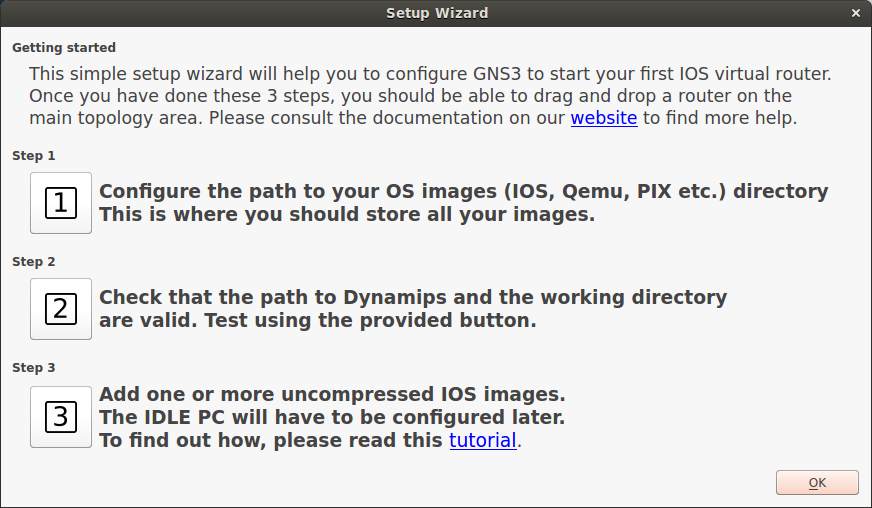
\includegraphics[scale=0.55]{res/pic001}
\caption{Мастер установки}
\end{figure}

От услуг этого мастера можно отказаться просто нажав "ОК" в правом нижнем углу.

Теперь перейдём к добавлению образов IOS. Их можно легко найти в интернете, на момент написания работы богатый выбор представлен на сайте \url{http://certs4u.info/ciscoios/c2650/c2691/}. Диалог добавления образа находится в меню Edit, пункт IOS images and hypervisors. Мы используем файл c2691-adventerprisek9\_sna-mz.124-13b.bin (это сжатый формат из которого можно получить c2691-adventerprisek9\_sna-mz.124-13b.image), а система автоматически определяет модель маршрутизатора (рис. 2).

\begin{figure}[h!]
\centering
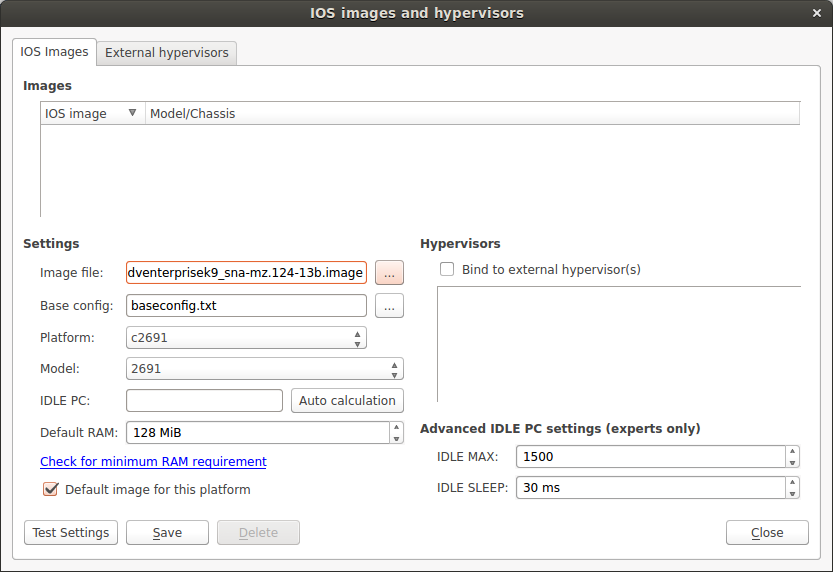
\includegraphics[scale=0.55]{res/pic002}
\caption{Диалог добавления образа IOS}
\end{figure}

Поле IDLE PC мы пока оставляем без внимания, вернёмся к нему позже.

Завершим работу диалога кнопкой Save и перейдём к диалогу создания нового проекта. Для его вызова, в меню File нужно выбрать пункт New blank project. В этом диалоге (рис. 3) важно выбрать пункт "Save nvrams including EtherSwitch VLANs and crypto keys".

\begin{figure}[h!]
\centering
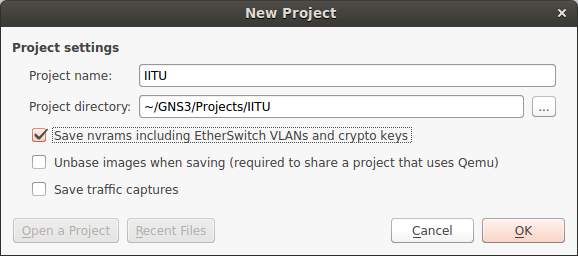
\includegraphics[scale=0.8]{res/pic003}
\caption{Диалог создания нового проекта}
\end{figure}

Этот пункт отвечает за сохранение конфигурации между перезапусками приложения.

Теперь добавим маршрутизатор на рабочую площадку (рис. 4) и запускаем его работу (пока с пустой конфигурацией).

\begin{figure}[h!]
\centering
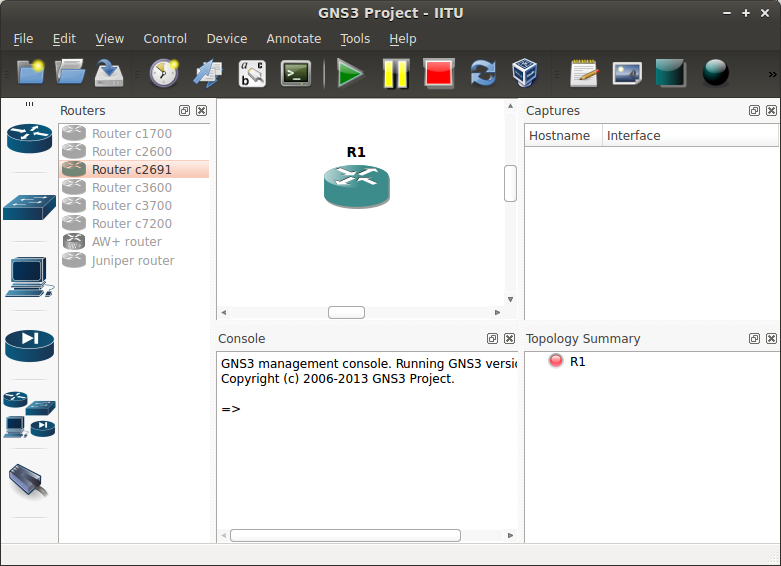
\includegraphics[scale=0.63]{res/pic004}
\caption{Диалог создания нового проекта}
\end{figure}

Это привело к колоссальной нагрузке на процессор -- 100\%!

\begin{Verbatim}[frame=single]
user@host:~$ top -b -n 1|grep dynamips
13909 user       20   0  553108 268408 197772 S 101,3  3,3   2:28.98 dynamips
\end{Verbatim}

Для оптимизации использования ресурсов процессов центрального процессора используется механизм IDLE PC, который мы ранее пропустили.

Его можно вызвать в контекстном меню, после чего система вычисляет несколько значений и предложит выбрать результат из списка. Рекомендуется выбирать значения со знаком * (рисунок 5). Как только они применяются, загрузка CPU падает (6,4\%).

\begin{Verbatim}[frame=single]
user@host:~$ top -b -n 1|grep dynamips
13909 user       20   0  553108 268408 197772 S   6,4  3,3  10:51.79 dynamips
\end{Verbatim}

\begin{figure}[h!]
\centering
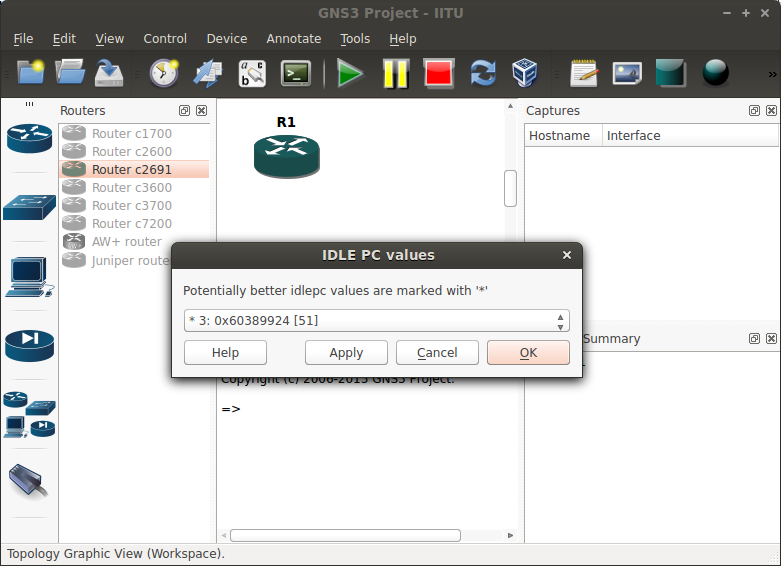
\includegraphics[scale=0.6]{res/pic005}
\caption{Оптимизация использования ресурсов CPU}
\end{figure}

Теперь можно подключиться к работающему роутеру. Для этого в контекстном меню нужно вызвать пункт console либо подключиться любим терминальным приложением к порту виртуального роутера через телнет. Номер порта можно узнать если навести мышку на роутер и немного подождать (рис. 6), либо через пункт Change console port контекстного меню.

\begin{figure}[h!]
\centering
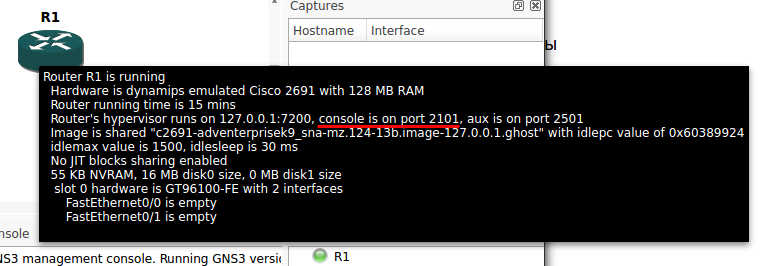
\includegraphics[scale=0.6]{res/pic006}
\caption{Определение номера порта консоли}
\end{figure}

Для подключения, нужно набрать команду
\begin{Verbatim}[frame=single]
telnet 127.0.0.1 2101
\end{Verbatim}

После чего появится доступ к управлению роутером (рис. 7).

\begin{figure}[h!]
\centering
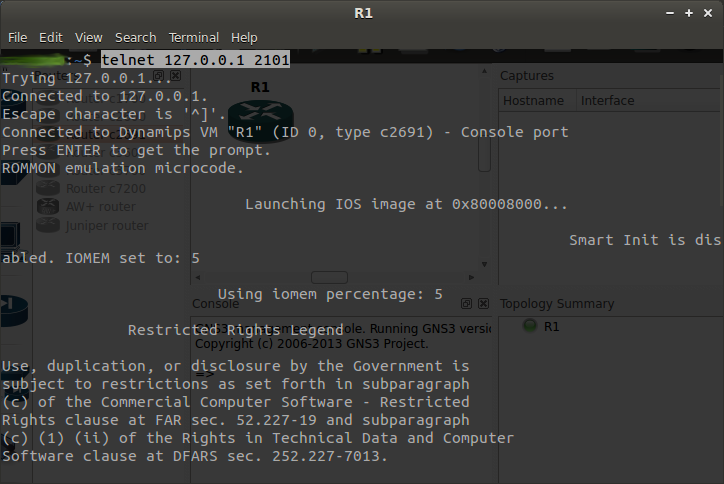
\includegraphics[scale=0.65]{res/pic007}
\caption{telnet подключение}
\end{figure}

%------------------------------------------------------------------------------
\newpage
\section{Виртуальные машины в эмулируемой сети}

GNS3 можно соединить с хостовой ОС Linux (на котором он запущен) и серверами в VirtualBox-е. Это значительно расширяет возможности по созданию сложных топологий с использованием роутеров Cisco, серверов с различными сервисами в VirtualBox и выходом в Интернет через хостовую ОС Linux. Виртуальные машины можно запускать и на QEMU, но VirtualBox предоставляет более удобный интерфейс для их создания и управления.

В данном примере используется сеть из трех соединенных между собой роутеров R1, R2 и R3, модели роутеров -- Cisco 2651XM. R1 через облако C1 подсоединен к родному хосту Ubuntu (на котором запущен GNS3). Для этой машины имя будет ubox. Через этот хост проводится синхронизация времени по ntp, закачка на роутеры дополнительных файлов по tftp и доступ в Интернет. Через облако С2 сеть подключена к виртуальной машине в VirtualBox. В данном случае это Debian с установленным FreeRADIUS для аутентификации и авторизации на роутерах и Syslog сервером для логов. Топология сети приведена на рисунке 8.

\begin{figure}[h!]
\centering
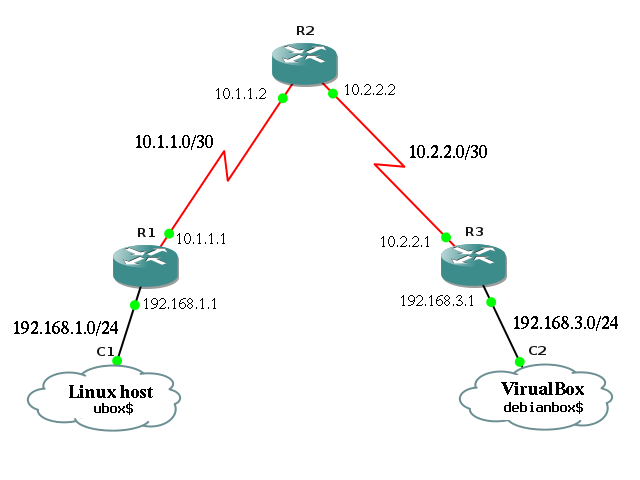
\includegraphics[scale=1]{res/pic008}
\caption{Топология сети}
\end{figure}

Для реализации этой схемы, произведём установку утилиты tunctl для создания и управления TUN/TAP виртуальными сетевыми интерфейсами:

\begin{Verbatim}[frame=single]
ubox$ sudo apt-get install -y uml-utilities
\end{Verbatim}

И утилиту brctl для создания и настройки сетевых мостов:
\begin{Verbatim}[frame=single]
ubox$ sudo apt-get install -y bridge-utils
\end{Verbatim}

Теперь создаем и конфигурируем виртуальные сетевые интерфейсы:
\begin{itemize}
\item tap0 -- для связи с Linux-ом, на котором и запущен GNS3.
\item tap1 -- для связи через мост с гостевыми машинами VirtualBox-а.
\end{itemize}
\begin{Verbatim}[frame=single]
ubox$ sudo tunctl -t tap0 -u username
ubox$ sudo tunctl -t tap1 -u username
ubox$ sudo ip addr add 192.168.1.1/24 dev tap0
ubox$ sudo ip link set up dev tap0
\end{Verbatim}

Обеспечим привязку интерфейсов к облаку (рис. 9)

\begin{figure}[h!]
\centering
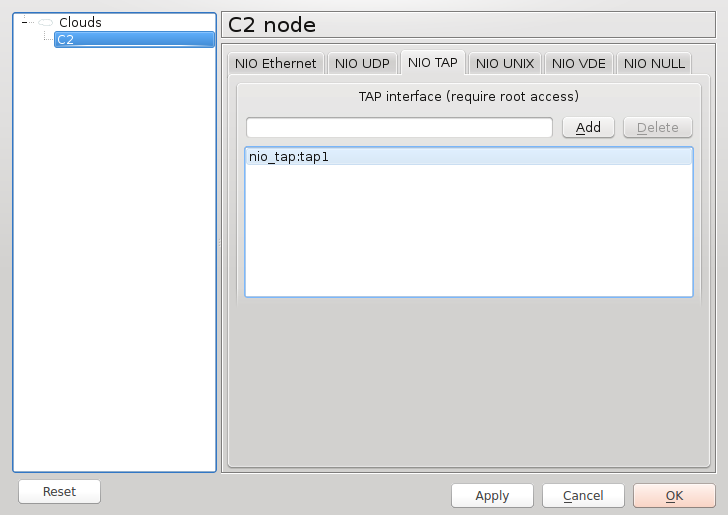
\includegraphics[scale=0.85]{res/pic009}
\caption{Привязка виртуальных интерфейсов}
\end{figure}

Связь с VirtualBox-ом осуществляется через мост br0, который состоит из виртуального Host-only интерфейса vboxnet0 и уже созданного tap1.
\begin{Verbatim}[frame=single]
ubox$ sudo brctl addbr br0
ubox$ sudo brctl addif br0 tap1
ubox$ sudo brctl addif br0 vboxnet0
ubox$ sudo ifconfig br0 192.168.3.4 netmask 255.255.255.0 up
\end{Verbatim}

Для связи всего этого хозяйства c хостовым Linux-ом на нем необходимо прописать маршрутизацию в используемые подсети:
\begin{Verbatim}[frame=single]
ubox$ sudo route add -net 10.1.1.0/24 gw 192.168.1.1
ubox$ sudo route add -net 10.2.2.0/24 gw 192.168.1.1
ubox$ sudo route add -net 192.168.3.0/24 gw 192.168.1.1
\end{Verbatim}

Теперь перейдём к настройке роутеров. На всех роутерах нужно прописать роутинг на подсети (или использовать протоколы динамической маршрутизации). Мы используем проприетарный цисковский протокол динамической маршрутизации EIGRP. Настройка выглядит следующим образом:

Для R1 --

\begin{Verbatim}[frame=single]
R1# conf t
R1(config)# router eigrp 1
R1(config-router)# passive-interface FastEthernet0/0
R1(config-router)# network 10.1.1.0 0.0.0.3
R1(config-router)# network 192.168.1.0
R1(config-router)# no auto-summary
R1(config-router)# exit
R1(config)# ip route 0.0.0.0 0.0.0.0 FastEthernet0/0
\end{Verbatim}

Для R2 --

\begin{Verbatim}[frame=single]
R2# conf t
R2(config)# router eigrp 1
R2(config-router)# network 10.1.1.0 0.0.0.3
R2(config-router)# network 10.2.2.0 0.0.0.3
R2(config-router)# no auto-summary
R2(config-router)# exit
R2(config)# ip route 0.0.0.0 0.0.0.0 Serial0/0
\end{Verbatim}

Для R3 --

\begin{Verbatim}[frame=single]
R3# conf t
R3(config)# router eigrp 1
R3(config-router)# passive-interface FastEthernet0/0
R3(config-router)# network 10.2.2.0 0.0.0.3
R3(config-router)# network 192.168.3.0
R3(config-router)# no auto-summary
R3(config-router)# exit
R3(config)# ip route 0.0.0.0 0.0.0.0 Serial0/0
\end{Verbatim}

На Debian-е (запущенном в VirtualBox) устанавливается сетевой адрес и шлюз по умолчанию:
\begin{Verbatim}[frame=single]
debianbox$ ifconfig eth0 192.168.3.3 netmask 255.255.255.0 up
debianbox$ route add default gw 192.168.3.1
\end{Verbatim}

Для того, чтобы работал Интернет через хостовый Linux нужно применить следующие правила (eth0 — внешний интерфейс).
\begin{Verbatim}[frame=single]
echo 1 > /proc/sys/net/ipv4/ip_forward
ubox$ sudo /sbin/iptables -t nat -A POSTROUTING -o eth0 -j MASQUERADE
ubox$ sudo /sbin/iptables -t nat -A POSTROUTING -o eth0 -j LOG
ubox$ sudo /sbin/iptables -A FORWARD -i eth0 -o tap0 -m state --state 
                                             RELATED,ESTABLISHED -j ACCEPT
ubox$ sudo /sbin/iptables -A FORWARD -i tap0 -o eth0 -j ACCEPT
\end{Verbatim}

На базе данного примера можно строить сетевые топологии еще больше и сложнее. GNS3 позволяет эмулировать ASA, PIX, IPS, JunOS; простые Ethernet, ATM и Frame Relay коммутаторы; позволяет перехватывать пакеты с помощью Wireshark.

%------------------------------------------------------------------------------

\newpage
\section{Анализ трафика}

%------------------------------------------------------------------------------

\newpage
\section*{Заключение}
\addcontentsline{toc}{section}{Заключение}



%------------------------------------------------------------------------------

\newpage
\section*{Список литературы}
\addcontentsline{toc}{section}{Список литературы}

\begin{enumerate}
\item Малышев И. А. - Методические указания по лабораторным работам по предмету «Администрирование компьютерных сетей».
\item Бешков А. VMware – виртуальный полигон для администратора и разработчика // Системный администратор, 2003, № 9.
\item Стахнов А. А. Сетевое администрирование Linux. – СПб: БХВ-Петербург, 2004.
\end{enumerate}

\end{document}